\documentclass[../main.tex]{subfiles}

\begin{document}

\section{Random Matrix Theory}
A lot of physical systems -- e.g. systems with glassy dynamics -- can often be modeled using graphs.
This makes graph theory an integral part of physics itself and it has been studied extensively.
In this exercise we will look at such systems that additionally contain disorder. 
Every regular graph can be expressed as an adjacency matrix which can be used to analyze the system.
\par

\subsection{Analysis by Direct Diagonalization}

\subsubsection{Sparse Random Matrix}
In the first step of our analysis we use well known techniques to establish a baseline for our methodology.
The method we use is called Direct Diagonalization and it obtains the spectrum of the system by using numeric Exact Diagonalization (ED).
\par 

\begin{figure}[htpb]
    \centering
    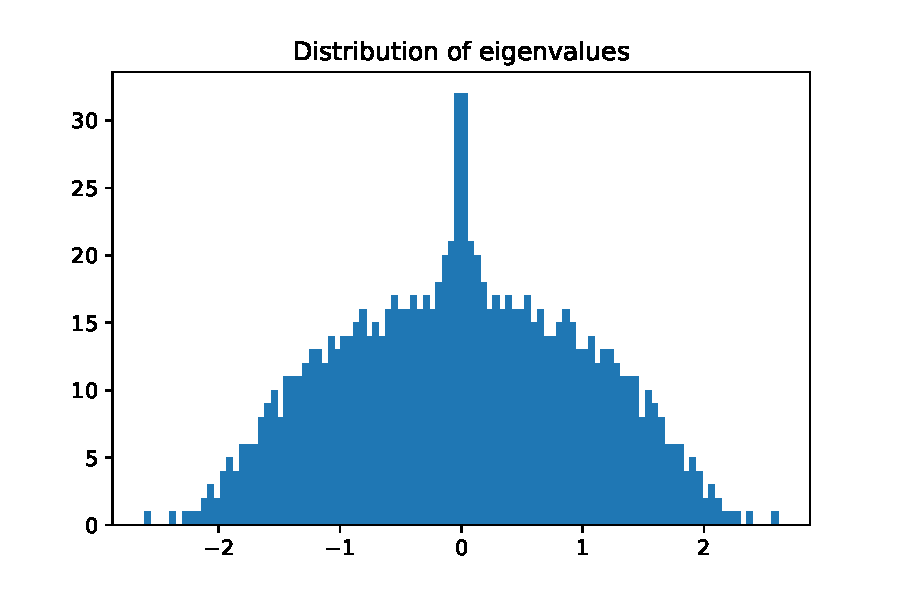
\includegraphics[width=0.8\textwidth]{../figures/2_1_1_spectrum_sparse.pdf}
    \caption{Spectrum of a RRG of size $2^{10}$ with connectivity 3 averaged over 10 different realizations.}
    \label{fig:spectrum_sparse}
\end{figure}

In a first analysis step we generate 10 different Random Regular Graphs (RRG) and calculate their spectrum vie ED and average their spectrum.
In Figure \ref{fig:spectrum_sparse} you can see the spectrum of the RRG's adjacency matrices of size $N = 2^{10}$ with connectivity 3 averaged over 10 different realizations.


\subsubsection{Fully Connected Graph}

Next we want to analyze the spectrum of a fully connected network. For this we gain generate an adjacency matrix multiply it's components with gaussian noise scaled by $c = N-1$.

\begin{figure}[htpb]
    \centering
    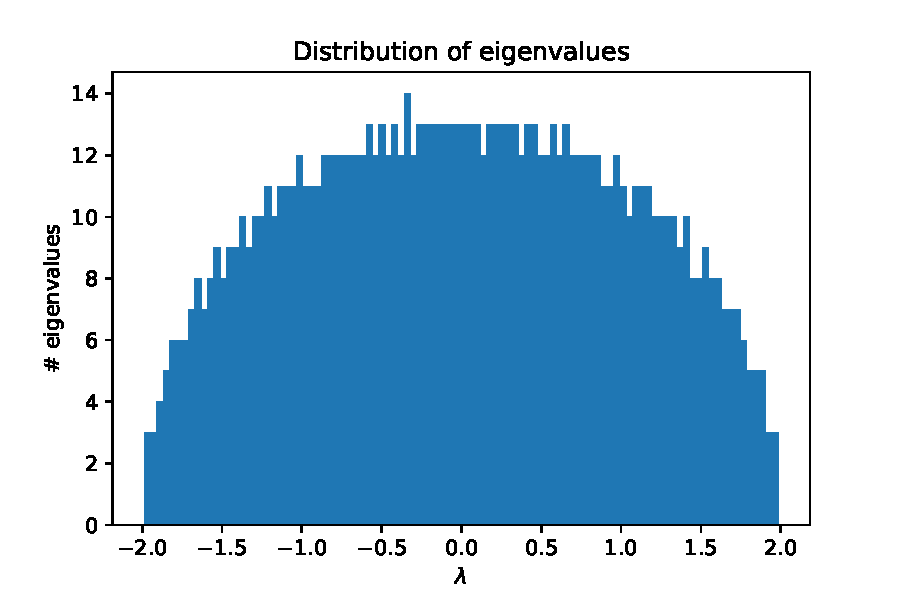
\includegraphics[width=0.8\textwidth]{../figures/2_1_2_spectrum_full.pdf}
    \caption{Spectrum of a fully connected network of size $N = 2^{10}$ ($c = N-1$) averaged over 10 different realizations.}
    \label{fig:spectrum_full}
\end{figure}

In Figure \ref{fig:spectrum_full} we can see the spectrum of the fully connected network averaged over 10 realizations of the Random Graph.



\subsubsection{Large Matrix limit}

As the number of nodes in the fully connected graph increases we expect the self-averaging effects of the system to become stronger.
This means that the density of our spectrum will more closely the exact solution in the $N\to \infty$ limit.
That solution is given by the Wigner-Semicircle law, which states that the density of eigenvalues describes a semicircle described by 

\begin{align}\label{eq:wigner_semicircle}
    \rho(\lambda) = \frac{\sqrt{4 - \lambda^2} }{2 \pi}
.\end{align}


\begin{figure}[htpb]
    \centering
    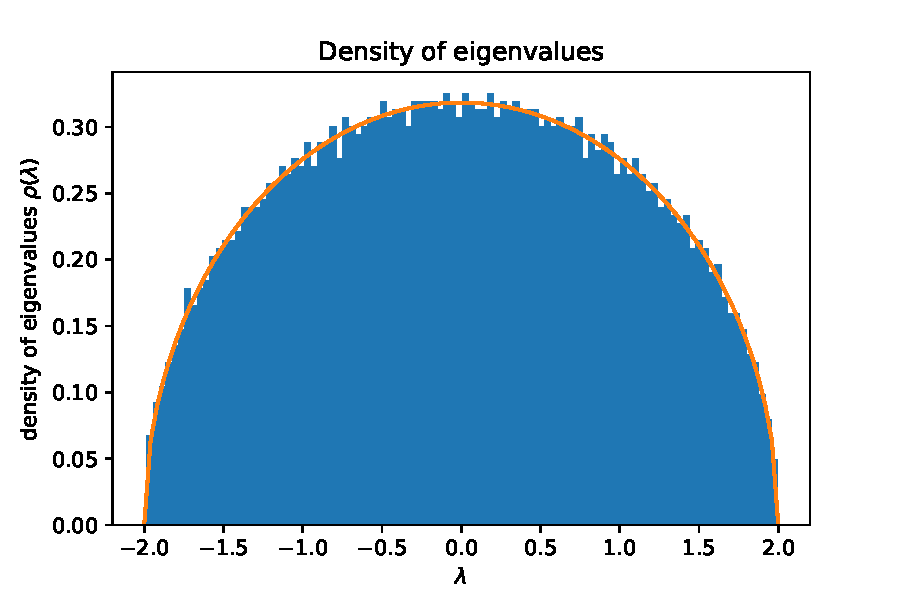
\includegraphics[width=0.8\textwidth]{../figures/2_1_3_wigner_semicircle.pdf}
    \caption{
        \emph{Spectral density} of a fully connected network of size $N= 2^{12}$ of a single realization of a single realization.
        Furthermore we overlayed the semicircle defined given by the Wigner-Semicircle law from eq. \eqref{eq:wigner_semicircle}.
    }
    \label{fig:wigner_semicircle}
\end{figure}

\subsubsection{Universality Classes}
As graphs with a high connectivity $c$ have very similar topology and their behavior is self-averaging, we can classify them by their spectral properties.

\begin{figure*}[htpb]
    \thisfloatpagestyle{empty}
    \vspace{-3cm}
    \centering
    \begin{subfigure}{\textwidth}
        \centering
        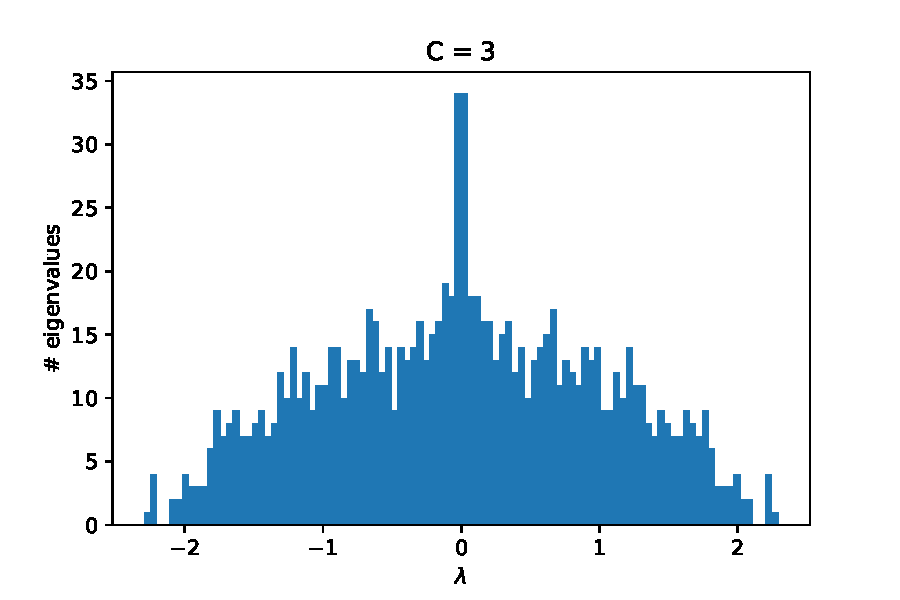
\includegraphics[width=.8\linewidth]{../figures/2_1_4_universality_classes0003.pdf}
        \caption{}
        \label{fig:universality_classes_0003}
    \end{subfigure}\\%
    \begin{subfigure}{\textwidth}
        \centering
        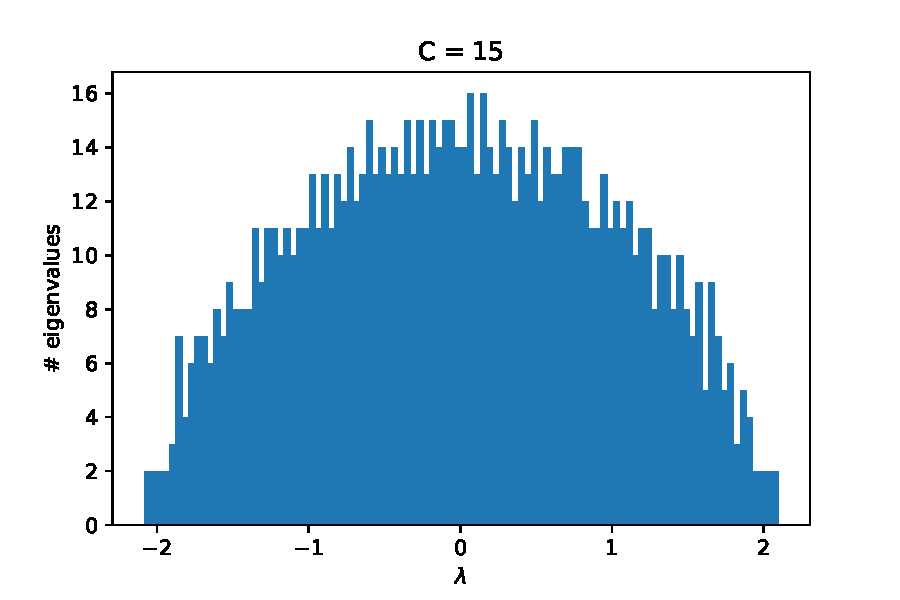
\includegraphics[width=.8\linewidth]{../figures/2_1_4_universality_classes0015.pdf}
        \caption{}
        \label{fig:universality_classes_0015}
    \end{subfigure}\\%
    \begin{subfigure}{\textwidth}
        \centering
        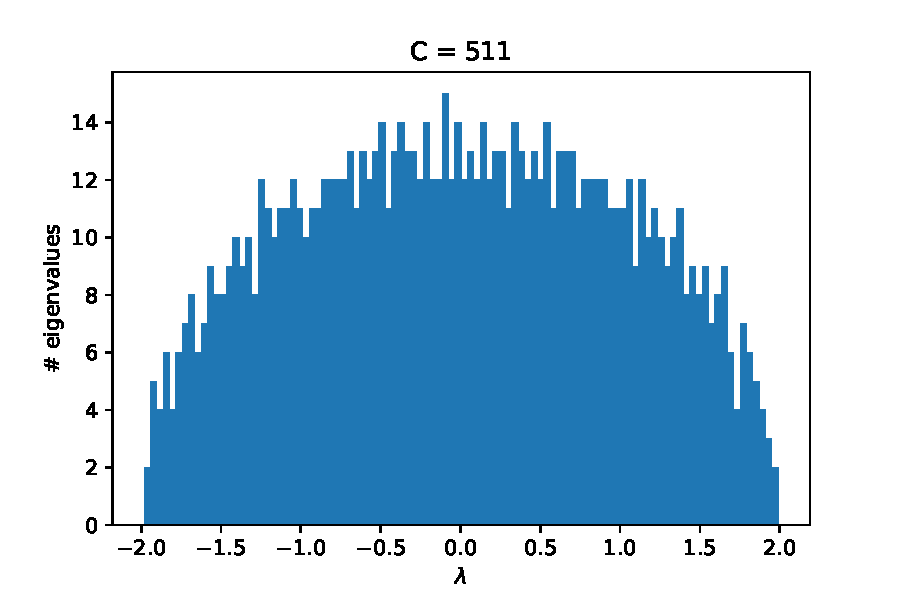
\includegraphics[width=.8\linewidth]{../figures/2_1_4_universality_classes0511.pdf}
        \caption{}
        \label{fig:universality_classes_0511}
    \end{subfigure}
    \caption{Spectrum of RRGs of size $N=2^{10}$ with different connectivities $c$.}
    \label{fig:universality_classes}
\end{figure*}

In Figures \ref{fig:universality_classes_0003}-\ref{fig:universality_classes_0511} we can see that already for quite small connectivities we get spectra that look very close to a semi-circle.
We can see that our idea that high connectivities should belong to the same class of spectrum does clearly hold.


\subsection{Analysis by Cavity Method}
\setcounter{subsubsection}{4}

\subsubsection{Update equation for the cavity precisions}

To calculate the cavity precisions of the Random Matrix problem we again impose gaussian distributions for our cavity and marginal probabilities.
This allows us to obtain recursive relations for the cavity and marginal precisions (inverse variances).

We can easily do so by inserting our assumptions into equations (18) and (19) on the exercise sheet.
The resulting equation for the cavity precision $\omega^{(j)}_k$ at some site $k$, given some cavity at site $j$ is 
\begin{align}
\label{eq:cavity_precs}
    \omega^{(j)}_k = i(\lambda - i \epsilon) + 
    \sum\limits_{l \in \partial k \setminus j }^{ } M^2_{ kl }/ \omega^{(k)}_l 
.\end{align}
$M_{ kl } $ is the value of the given random adjacency matrix representing the edge between site $k$ and $l$.

In similar fashion we can also obtain an equation for the marginal precisions $\omega_k$ at site $k$
\begin{align}
\label{eq:marginals_precs}
    \omega_k = i(\lambda - i \epsilon) + 
    \sum\limits_{l \in \partial k}^{ } M^2_{ kl }/ \omega_l 
.\end{align}

\subsubsection{Cavity method for sparse matrices}

\begin{figure}[htpb]
    \centering
    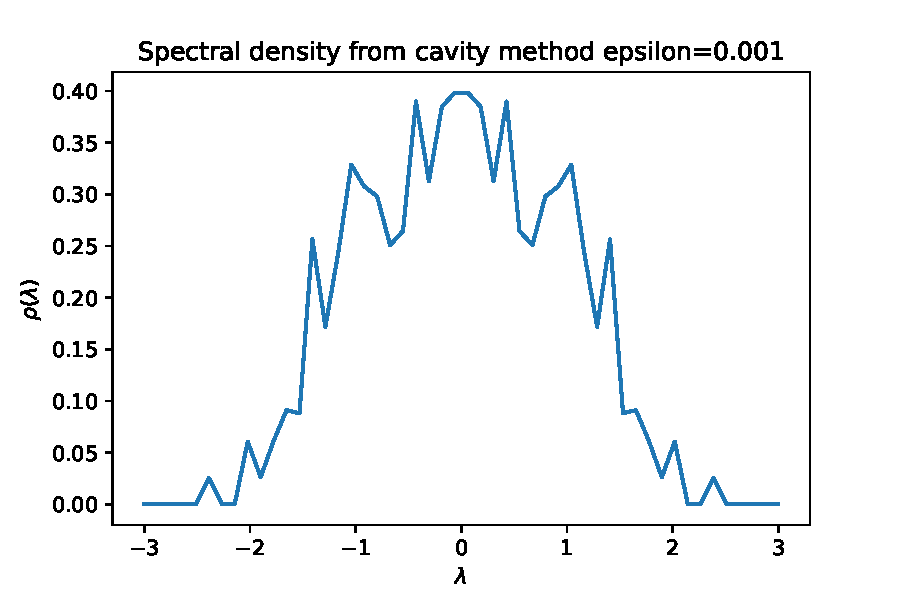
\includegraphics[width=0.8\textwidth]{../figures/ex2_spectrum_eps_large.pdf}
    \caption{
        Spectral density calculated from the Cavity Method for $\varepsilon=\num{e-3}$ in a sparsely connected RRG of connectivity $c = \num{3}$.
        The graph is made up from $\num[parse-numbers = false]{2^{11}}$ nodes.
    }
    \label{fig:rrg_spectrum_cavity}
\end{figure}

\begin{figure}[htpb]
    \centering
    \begin{subfigure}{.5\textwidth}
        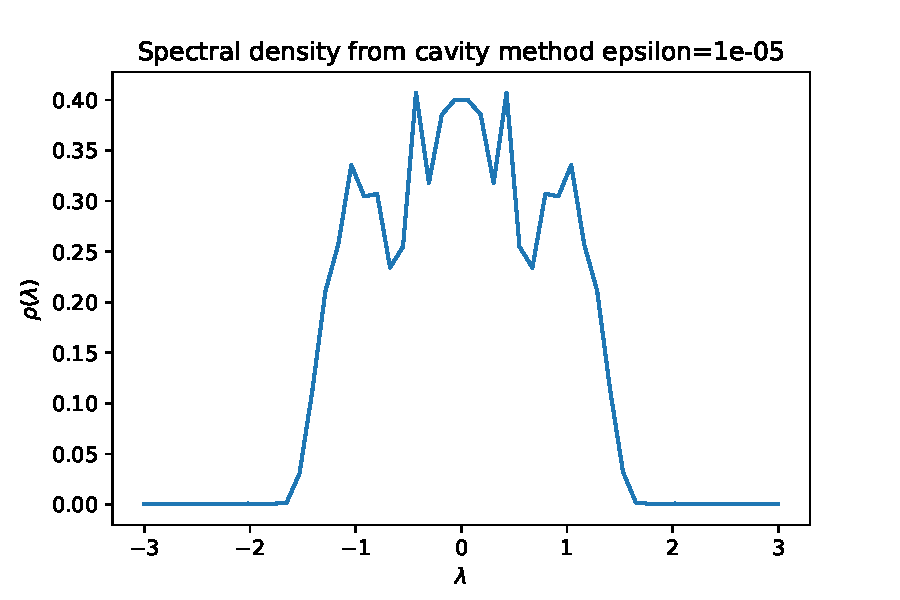
\includegraphics[width=\textwidth]{../figures/ex2_spectrum_eps_medium.pdf}
        \caption{}\label{fig:rrg_spectrum_eps_med}
    \end{subfigure}%
    \begin{subfigure}{.5\textwidth}
        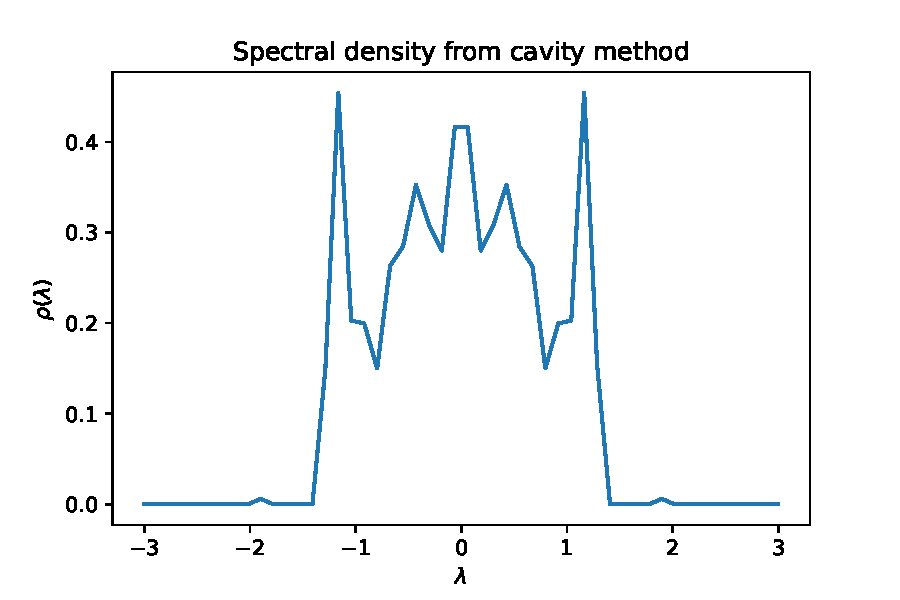
\includegraphics[width=\textwidth]{../figures/ex2_spectrum_eps_small.pdf}
        \caption{}\label{fig:rrg_spectrum_eps_small}
    \end{subfigure} 
    \caption{
        Spectrum of the system for different parameters of $\varepsilon =$ \num{e-5}(\num{e-8}) in figure \subref{fig:rrg_spectrum_eps_med}/\subref{fig:rrg_spectrum_eps_small}.
        Similar to Figure \ref{fig:rrg_spectrum_cavity} the size of the graph is \num[parse-numbers = false]{2^{11}} and the connectivity is $c = 3$.
    }
    \label{fig:rrg_spectrum_different_eps}
\end{figure}

Next to the method of direct Diagonalization we can also use the cavity method to obtain the spectrum of the graph's adjacency matrix.
The spectrum shown in Figure \ref{fig:rrg_spectrum_cavity} was obtained using this method using the cavity equations \eqref{eq:cavity_precs} and \eqref{eq:marginals_precs}.
We find that the spectrum is qualitatively consistent with the results obtained from Direct Diagonalization in Figure \ref{fig:spectrum_sparse}.
\par

In Figure \ref{fig:rrg_spectrum_different_eps} we have displayed that same spectrum calculated using the cavity method but for different values of $\varepsilon$.
We can see that the spectra from this version of the algorithm are slightly different to the one obtained for a larger $\varepsilon$.
As to what the role of $\varepsilon$ in the algorithm we feel that these results are inconclusive.
Nonetheless we suspect that $\varepsilon$ influences the convergence behavior of the algorithm and both Plots in Figure \ref{fig:rrg_spectrum_different_eps} show poorly converged spectra.
\par

\subsubsection{Mean-Field limit}
\label{sec:mean_field_limit}

In the mean-field limit for the fully connected graph we assume $N \to \infty$.
We can see from equation \eqref{eq:cavity_precs} that -- in this limit and on a fully connected graph -- the single term left out scales as $\mathcal{O}(1)$, while the entire sum scales as $\mathcal{O}(N)$.
As $N$ grows, we will find that it will be increasingly less significant whether we will be looking at the marginals or the cavity distributions.

\subsubsection{Mean Resolvent}

Another means to verify our results is by analyzing the system analytically in the mean field limit introduced in Section \ref{sec:mean_field_limit}.
We do so by analyzing the mean resolvent $g$ and expressing it in terms of the marginal precisions $\omega_j$
\begin{align}
    \label{eq:mean_resolvent}
    g_{ \text{MF} } = \frac{i}{N}\sum_{j=1}^{N} \omega_j^{-1}
.\end{align}

Into equation \eqref{eq:mean_resolvent} we the obtained recursive relationship for the marginal precisions from equation \eqref{eq:marginals_precs}.
By using that $A_{ ij } = 1$ in $M_{ ij } = A_{ ij } J_{ ij } $ we can simplify the obtained equation to get 
\begin{align}
    \label{eq:mean_resolvent_limit}
    g_{ \text{MF} }  = \frac{i}{N} \sum_{j=1}^{N} \left( i(\lambda - i \varepsilon) + \sum_{k \in \partial j}^{} \frac{J^2_{ kj }}{\omega_k} \right)^{-1}
.\end{align}

As we are using the fully connected case we can resolve the sum inside the parenthesis in equation \eqref{eq:mean_resolvent_limit} to obtain 
\begin{align}
    \label{eq:mean_resolvent_resolved}
    g_{ \text{MF} } = \frac{1}{N} \sum_{j=1}^{N} \frac{1}{i(\lambda - i \varepsilon) + \frac{1}{N}\sum\limits_{k}^{N} \frac{1}{\omega_k}}
.\end{align}

Such we have found the self-consistent equation (by identifying the sum of the denominator in equation \eqref{eq:mean_resolvent_resolved} with $g_{ \text{MF} } $).
This equation is nothing more than then a quadratic equation in the mean field resolvent 

\[
    g_{ \text{MF} } = \frac{i}{i(\lambda - i \varepsilon) - i g_{ \text{MF} } }  
    \qquad 
    \Longleftrightarrow
    \qquad
    g_{ \text{MF} } = \frac{\lambda_\varepsilon}{2} \pm \sqrt{\frac{\lambda_\varepsilon^2}{4} - 1}, 
    \qquad
    \lambda_\varepsilon = \lambda - i \varepsilon
.\] 

If we plug this result into the given equation for the spectral density we recover the Wigner-Semicircle law 

\[
    \rho(\lambda) = \lim\limits_{\varepsilon \to 0} \operatorname{Im}\left(\frac{\lambda_\varepsilon}{2} \pm\sqrt{\frac{\lambda_\varepsilon^2}{4} - 1}\right) = \frac{1}{2\pi} \sqrt{4 - \lambda^2} 
.\] 

Such we have shown that our simulation techniques are indeed consistent with analytical results.


\ifSubfilesClassLoaded{
	% if it's compiled alone
}{
	% if it's compiled in the main file
    \newpage
}
\end{document}
